% ============================================================
% §1  Introduction
% ============================================================

\section{Introduction}
\label{sec:intro}

Real-world cyber-physical systems --- water treatment plants, server clusters, spacecraft telemetry arrays --- continuously generate high-dimensional sensor streams whose reliable anomaly detection prevents safety incidents and operational losses~\cite{schmidl2022evaluation,blazquez2021review}.
Anomalies in such streams manifest not in isolated channels but through correlated deviations across multiple sensor dimensions~\cite{deng2021gdn,wu2025catch}.
Because exhaustive point-level annotation of anomalies is infeasible at scale, the dominant paradigm for multivariate time series anomaly detection (MTSAD) has been unsupervised learning~\cite{wang2025nrdetector}.

The resulting body of work spans four broad families --- reconstruction-based~\cite{zong2018dagmm,su2019omnianomaly,audibert2020usad,song2023memto,wu2025catch}, prediction-based~\cite{deng2021gdn}, association-discrepancy and contrastive~\cite{xu2022anomalytransformer,yang2023dcdetector}, and backbone-based~\cite{tuli2022tranad,wu2023timesnet} methods (Section~\ref{sec:related_mtsad}) --- that, despite their differences, all treat the training data as drawn entirely from normal operations.
These methods consequently have no mechanism for exploiting labeled anomalies even when such labels are available: the best a label-aware variant can do is exclude confirmed anomaly windows from training, filtering contamination rather than learning from it~\cite{wang2025nrdetector}.

In practice, however, a small fraction of training observations carry anomaly labels, typically from recorded fault and attack events in operational logs~\cite{wang2025nrdetector}.
These labeled anomalies are contamination for unsupervised methods but a valuable learning signal for semi-supervised ones.
This label gap is particularly acute in the standard MTSAD benchmarks evaluated here: their original training splits contain no labeled anomalies by construction (per-dataset label semantics in \ref{sec:appendix_dataset}).
Benchmark studies have independently criticized dataset and evaluation practices in this field~\cite{liu2024elephant,schmidl2022evaluation}.
Evaluating any method that exploits labeled anomalies therefore requires modifying the data partition, as detailed in Section~\ref{sec:datasets}.

Our key observation is that labeled anomalies reveal three distinct learning signals: (a) which temporal positions serve as informative hard reconstruction targets, (b) which patches the Student decoder should avoid mimicking, and (c) what representational content should be adversarially suppressed in the Student's encoding.
The design exploits all three simultaneously to amplify both the reconstruction error and the Teacher--Student discrepancy at anomalous regions (Section~\ref{sec:ablation}).
Relying only on (b) is insufficient.
A Student repeatedly exposed to anomalous patterns during training may learn to reconstruct them accurately via an indirect pathway, weakening the discrepancy signal at inference time; the adversarial suppression of (c) closes this pathway at the representational level.
The closest prior work on deep semi-supervised MTSAD, NRdetector~\cite{wang2025nrdetector}, delegates representation learning to a label-agnostic pre-trained backbone, leaving labels unable to shape the representations themselves.

% ---- Figure 1: Setting-comparison diagram ----
\begin{figure}[tbp]
  \centering
  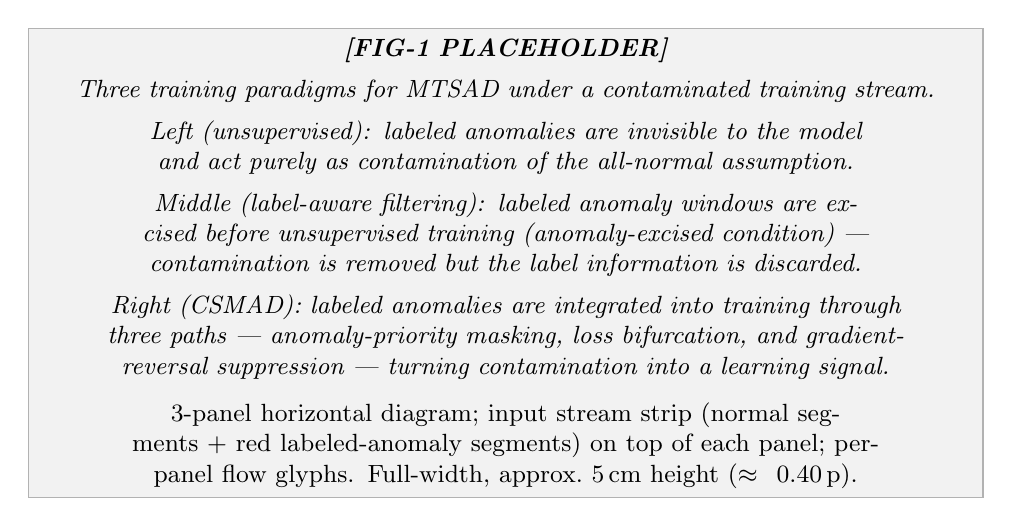
\begin{tikzpicture}
    \node[draw=gray!60, fill=gray!10, minimum width=\linewidth, minimum height=4.8cm,
          text width=0.92\linewidth, align=center, font=\small\itshape] (box) {%
      \textbf{[FIG-1 PLACEHOLDER]}\\[4pt]
      Three training paradigms for MTSAD under a contaminated training stream.\\[4pt]
      \textit{Left (unsupervised):} labeled anomalies are invisible to the model and act purely
      as contamination of the all-normal assumption.\\[4pt]
      \textit{Middle (label-aware filtering):} labeled anomaly windows are excised before
      unsupervised training (anomaly-excised condition) ---
      contamination is removed but the label information is discarded.\\[4pt]
      \textit{Right (CSMAD):} labeled anomalies are integrated into training through three
      paths --- anomaly-priority masking, loss bifurcation, and gradient-reversal suppression
      --- turning contamination into a learning signal.\\[6pt]
      \normalfont 3-panel horizontal diagram; input stream strip (normal segments + red
      labeled-anomaly segments) on top of each panel; per-panel flow glyphs.
      Full-width, approx.\ 5\,cm height ($\approx 0.40$\,p).
    };
  \end{tikzpicture}
  \caption{Three training paradigms for multivariate time series anomaly detection under a
    contaminated training stream.
    \textit{Left (unsupervised)}: labeled anomalies are invisible to the model and act purely
    as contamination of the all-normal assumption.
    \textit{Middle (label-aware filtering)}: labeled anomaly windows are excised before
    unsupervised training (the anomaly-excised condition; \S\ref{sec:baselines}) ---
    contamination is removed but the label information is discarded.
    \textit{Right (CSMAD)}: labeled anomalies are integrated into training through three
    paths --- anomaly-priority masking, loss bifurcation, and gradient-reversal suppression
    --- turning contamination into a learning signal.}
  \label{fig:setting}
\end{figure}

Building on these observations, we propose \textbf{CSMAD} (Contaminated Semi-supervised Masked Anomaly Detector), an end-to-end framework that integrates labeled anomaly information directly into masked autoencoder representation learning.
CSMAD employs, to our knowledge, the first architecture combining masked-reconstruction self-distillation with gradient reversal to adversarially suppress anomaly-specific information from the Student's representation in a contaminated semi-supervised MTSAD setting.
(Earlier semi-supervised models for time series integrate labels through loss terms attached to a generative or predictive objective, not adversarially through the gradient of the representation itself~\cite{xue2022fewpositive,huang2022slavae}; Section~\ref{sec:related_semi}.)
Our contributions are as follows:

\begin{enumerate}
  \item \textbf{Contaminated semi-supervised setting and benchmark protocol.}
    We formalize the \emph{contaminated semi-supervised} setting, in which labeled anomalies coexist with unlabeled training windows, and introduce a benchmark protocol that incorporates the chronological prefix of each dataset's test stream into training.
    The protocol constructs training splits containing labeled anomalies absent from the original splits and evaluates on the held-out temporal suffix.

  \item \textbf{Three-path label integration into masked autoencoder representation learning.}
    CSMAD integrates labeled anomalies through three orthogonal mechanisms:
    (i) \emph{anomaly-priority masking}, which selects labeled anomaly patches for reconstruction with highest priority, preventing the model from evading hard positions;
    (ii) \emph{loss bifurcation}, which restricts the Student decoder's imitation objective to normal-patch outputs;
    and (iii) \emph{gradient-reversal suppression}, which adversarially removes anomaly-specific information from the Student's internal representation via a reversed-gradient anomaly classifier.

  \item \textbf{Asymmetric Teacher--Student decoder architecture.}
    A deeper Teacher decoder (3 layers) establishes a stable normal-reconstruction reference, while a capacity-limited Student decoder (2 layers) fails more severely on anomalous correlation patterns than on normal ones --- a design intended to make the Teacher--Student output discrepancy a reliable anomaly signal under contaminated training (quantified in \ref{sec:extended_ablations}).

  \item \textbf{Extensive empirical evaluation.}
    Experiments on [N] multivariate datasets covering industrial control, IT infrastructure, and spacecraft telemetry demonstrate competitive performance against [N] baselines under five evaluation metrics, with the label sparsity sweep confirming that detection degrades gradually toward the unsupervised floor.
    % PH:NUM-004 | dataset-family count (sync with NUM-001)
    % PH:NUM-005 | total baseline count (sync with NUM-002)
\end{enumerate}

%% D-013: standard roadmap transition sentence removed (pure navigation, duplicated
%% by section headings; see PROSE_DIFF_LOG.md §D-013 entry 1.4)

%% PDF QA r1 MAJOR-8: keep this section's floats from drifting past the section end
\BodyFloatBarrier
